\documentclass[12pt,oneside,openright,a4paper,english,brazil]{abntex2}

\usepackage[utf8]{inputenc}
\usepackage{amsmath}
\usepackage{esint}
\usepackage{lmodern}
\usepackage{lipsum}
\usepackage{babel}
\usepackage{graphicx}
\usepackage[T1]{fontenc}
\usepackage{indentfirst}
\usepackage{amsfonts}
\usepackage{amssymb}
\usepackage{microtype}
\usepackage{color}
\usepackage[brazilian,hyperpageref]{backref}
\usepackage[alf]{abntex2cite}
\usepackage{xcolor}
\usepackage{graphicx}


\renewcommand{\backrefpagesname}{Citado na(s) página(s):~}
\renewcommand{\backref}{}
\renewcommand*{\backrefalt}[4]{
	\ifcase #1
	Nenhuma citação no texto.
	\or
	Citado na página #2.
	\else
	Citado #1 vezes nas páginas #2.
	\fi}


\titulo{LISTA DE EXERCÍCIOS 2}
\autor{MAXUEL RIBEIRO CASSINHA}
\data{Junho de 2020}
\instituicao{UNIVERSIDADE DE SÃO PAULO -- USP \par ESCOLA DE ENGENHARIA DE LORENA -- EEL}
\local{LORENA,SP}
\preambulo{LISTA DE EXERCÍCIOs DO MINICURSO DE LaTeX APRESENTADO À LABEEL}

\makeatletter
	\hypersetup{
		pdftitle={\@title},
		pdfauthor={\@author},
		pdfsubject={\imprimirpreambulo},
		pdfcreator={LaTeX with abnTeX2},
		pdfkeywords={abnt}{latex}{abntex}{abntex2}{relatório técnico},
		colorlinks=true,
		linkcolor=blue,
		citecolor=blue,
		filecolor=magenta,
		urlcolor=blue,
		bookmarksdepth=4
	}
\makeatother
\setlength{\parindent}{1.3cm}


\setlength{\parskip}{0.2cm}
\makeindex

\begin{document}
\selectlanguage{brazil}

\frenchspacing
\imprimircapa
\imprimirfolhaderosto

\centerline{\textbf{PROBLEMA 1}}
\par
\textbf{2.(a)}

\begin{equation}
    \begin{cases}
    \frac{\mathrm{d}x}{\mathrm{d}t}=\sigma(y-x)\\
    \frac{\mathrm{d}y}{\mathrm{d}t}=x(p-z)-y\\
    \frac{\mathrm{d}z}{\mathrm{d}t}=xy-\beta z
    \end{cases}
\end{equation}

\textbf{1.(a)}

\begin{equation}
    \mathrm{F}(k)=\frac{1}{2\pi}\int^\infty_{-\infty}\mathrm{s}(x)e^{ikx}\mathrm{d}x
\end{equation}


\clearpage
\centerline{\textbf{PROBLEMA 2}}

\textbf{TABELA IBGE}

\begin{table}[htb]
\IBGEtab{
\caption{Um Exemplo de tabela conforme padrão IBGE.} \label{tab:ibge} }
{ \begin{tabular}{ccc}
\toprule
QTD & ESTOQUE & VALOR \\
\midrule \midrule
12141820 & 205679 & 1687,48 \\
\midrule
15687610 & 987875 & 1984,00 \\
\midrule
12345678 & 125689 & 2002,90 \\
\bottomrule
\end{tabular} }
{ \fonte{AUTOR} }
\end{table}

\textbf{OUTRA FORMATAÇÃO DE TABELA}
\begin{table}[htb]
\begin{center}
\ABNTEXfontereduzida
\caption[<como aparece na lista de tabelas>]{\label{tab:formal} Tabela em outra formatação}
\begin{tabular}{m{2.6cm}|m{4.0cm}|m{2.25cm}|m{3.40cm}}
\hline
\textbf{QTD} & \textbf{ESTOQUE} & \textbf{VALOR} \\ \hline
 12141820 & 205679 & 1687,48  \\
 \hline
 15687610 & 987875 & 1984,00 \\
 \hline
12345678 & 125689 & 2002,90\\
\hline
\end{tabular}
\legend{Fonte: AUTOR}
\end{center}
\end{table}

\clearpage
\centerline{PROBLEMA 3}



\begin{figure}[!htb]
  \begin{center}
    \caption{\label{fig:Lorenzatt}Atrator de Lorenz}
    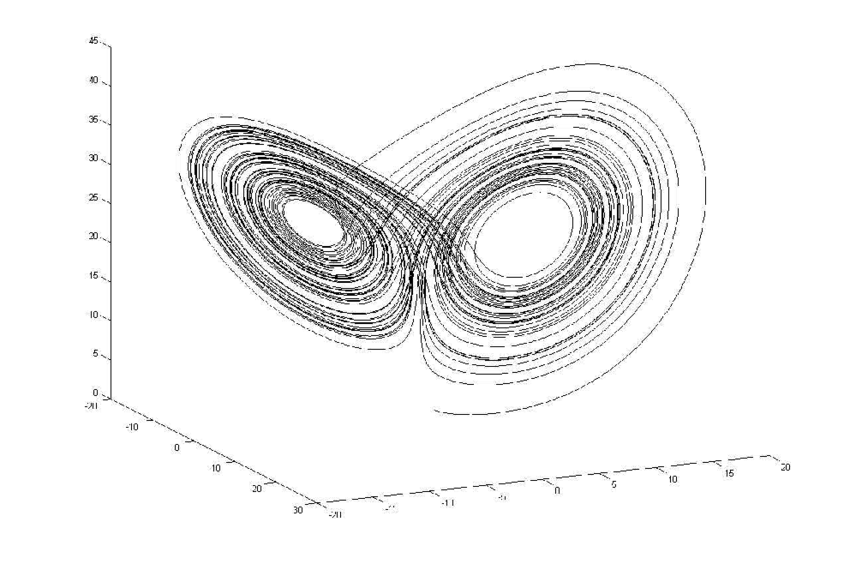
\includegraphics[scale=0.2, width=0.85\textwidth,height=0.65\textheight]{./atrator.png}
    \legend{Fonte: Wordpress}
  \end{center}
\end{figure}

\end{document}



%%% Local Variables:
%%% mode: latex
%%% TeX-master: t
%%% End:
